% Annexe B
\myChapter{Analyses causales complémentaires}{Analyses causales complémentaires}
\label{annexe:analyses-causales}
\mySaveMarks

\mySectionStar{Analyse causale étendue}{}{false}
\label{ssec:exp-annexe-causal-ext}

La Fig.~\ref{fig:exp-interventions} cartographie la réponse aux perturbations contrôlées $\Delta q+20\,\%$ et $\Delta t+3$~K. La comparaison entre le DAG appris $\Adag$ et le DAG physique de référence (couplage quasi-géostrophique descendant) donne deux arêtes sur cinq physiquement attendues correctement orientées ($Q_{\mathrm{phys}}=0{,}40$).

\begin{figure}[H]
\centering
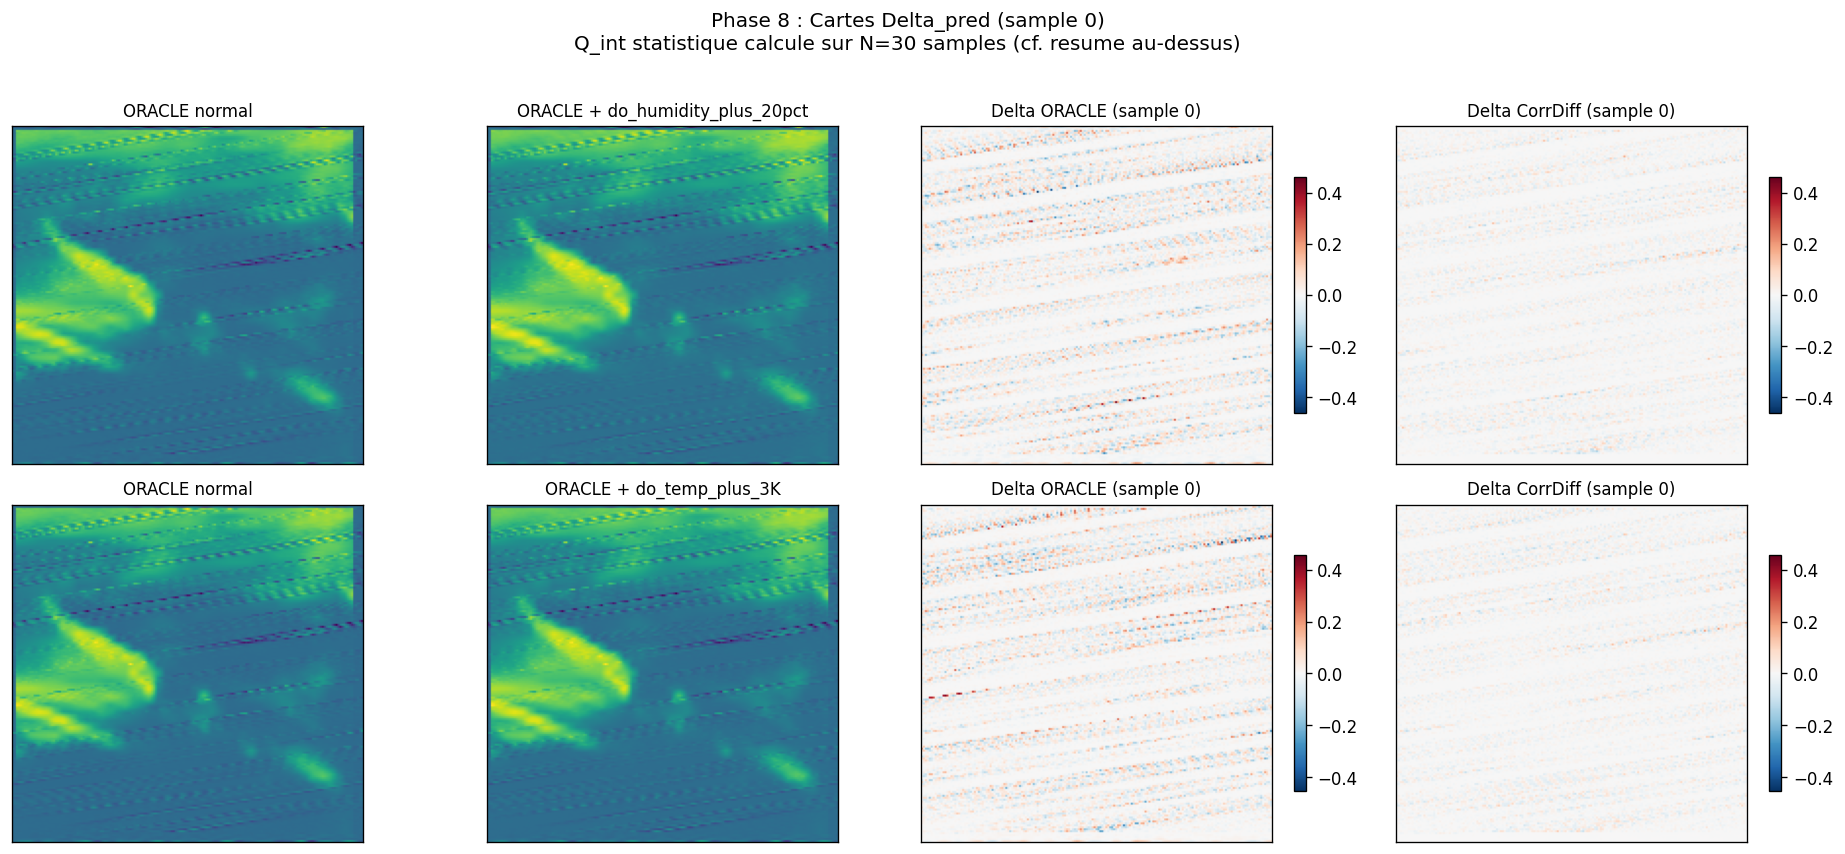
\includegraphics[width=0.85\linewidth]{../results/v5_evaluation/phase8_figures/03_interventions_maps.png}
\caption[Cartes des perturbations contrôlées]{Cartes des perturbations contrôlées $\Delta q+20\,\%$ et $\Delta t+3$~K. Signes physiques cohérents avec la relation de Clausius-Clapeyron sur les deux perturbations testées. Les amplitudes, de l'ordre de $10^{-3}$ en unités relatives, rendent les cartes visuellement peu contrastées : les statistiques quantitatives (moyennes et IC bootstrap) figurent au Tableau~\ref{tab:exp-res-int}.}
\label{fig:exp-interventions}
\end{figure}

\begin{figure}[H]
\centering
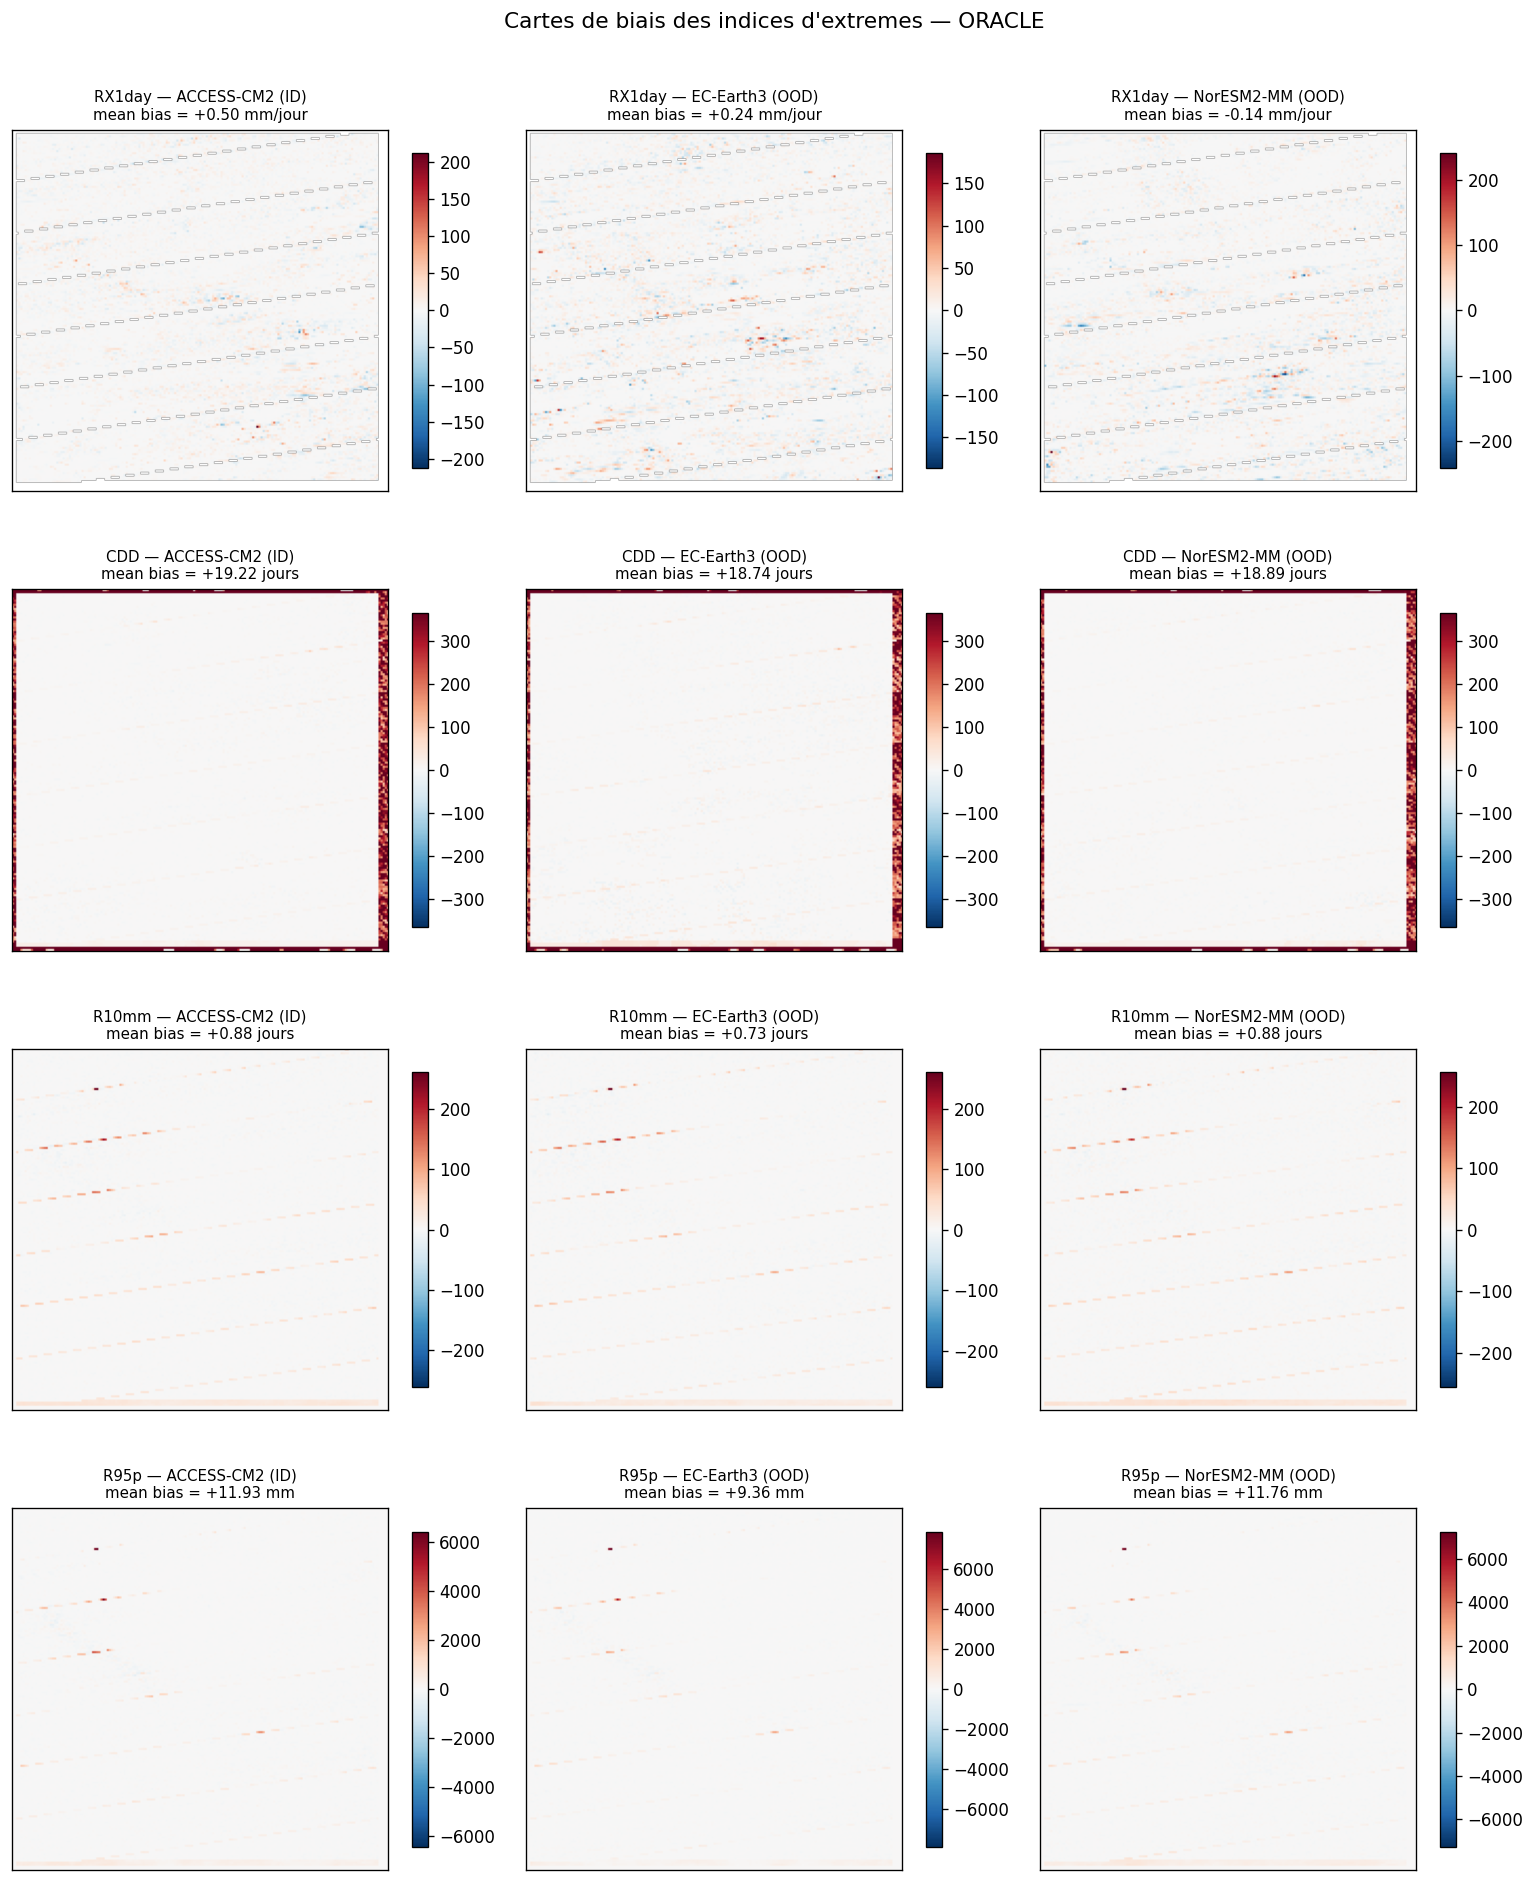
\includegraphics[width=0.78\linewidth]{../results/v5_evaluation/phase10_extreme_bias_maps/extreme_bias_ORACLE.png}
\caption[Biais RX1day d'Oracle]{Biais sur l'indice RX1day pour \Oracle{}. Le déficit, concentré sur le versant occidental des Southern Alps, révèle l'absence d'orographie HR (DEM) en entrée. Le même schéma spatial s'observe sur \CorrDiff{}, ce qui montre que la cause est l'information manquante, pas la causalisation. La rangée RX1day porte l'essentiel du message ; les autres indices sont donnés pour complétude, chaque carte ayant sa propre échelle de couleur.}
\label{fig:exp-extreme-bias-oracle}
\end{figure}

\mySectionStar{Variante à 9 nœuds (récupération structurelle)}{}{false}
\label{ssec:exp-annexe-9node}

La variante à 9 nœuds attribue un nœud à chaque variable atmosphérique : la chaîne sèche quasi-géostrophique (GP850, GP500, GP250, plus les méta-paths GP850$\to$GP500 et GP500$\to$GP250) est complétée par la chaîne humide de Held-Soden (Q850, W500, IVT), puis fermée sur la précipitation de surface SP\_HR. Elle est entraînée sous le \emph{même} protocole two-stage que la configuration principale (split temporel 1980--2009 / 2010--2011 / 2012--2013, 215 époques, seed 42).

La matrice $\Adag$ apprise (Fig.~\ref{fig:exp-9node-dag}) récupère les \textbf{dix} arêtes physiquement attendues avec le signe correct et sans arête parasite ($n_{\mathrm{extra}}=0$), pour un score de fidélité continu $Q_{\mathrm{phys}}=0{,}9997$ (binaire $1{,}0$) et un squelette parfait (\texttt{skeleton\_F1}$=1{,}0$) ; le détail arête par arête figure au Tableau~\ref{tab:exp-9node-edges}. Les magnitudes restent quasi uniformes (environ $0{,}69$) : la structure est \emph{fidèlement orientée} sans être hiérarchisée en amplitude, ce qui reste cohérent avec la limite d'identifiabilité observationnelle d'un SCM.

\begin{figure}[H]
\centering
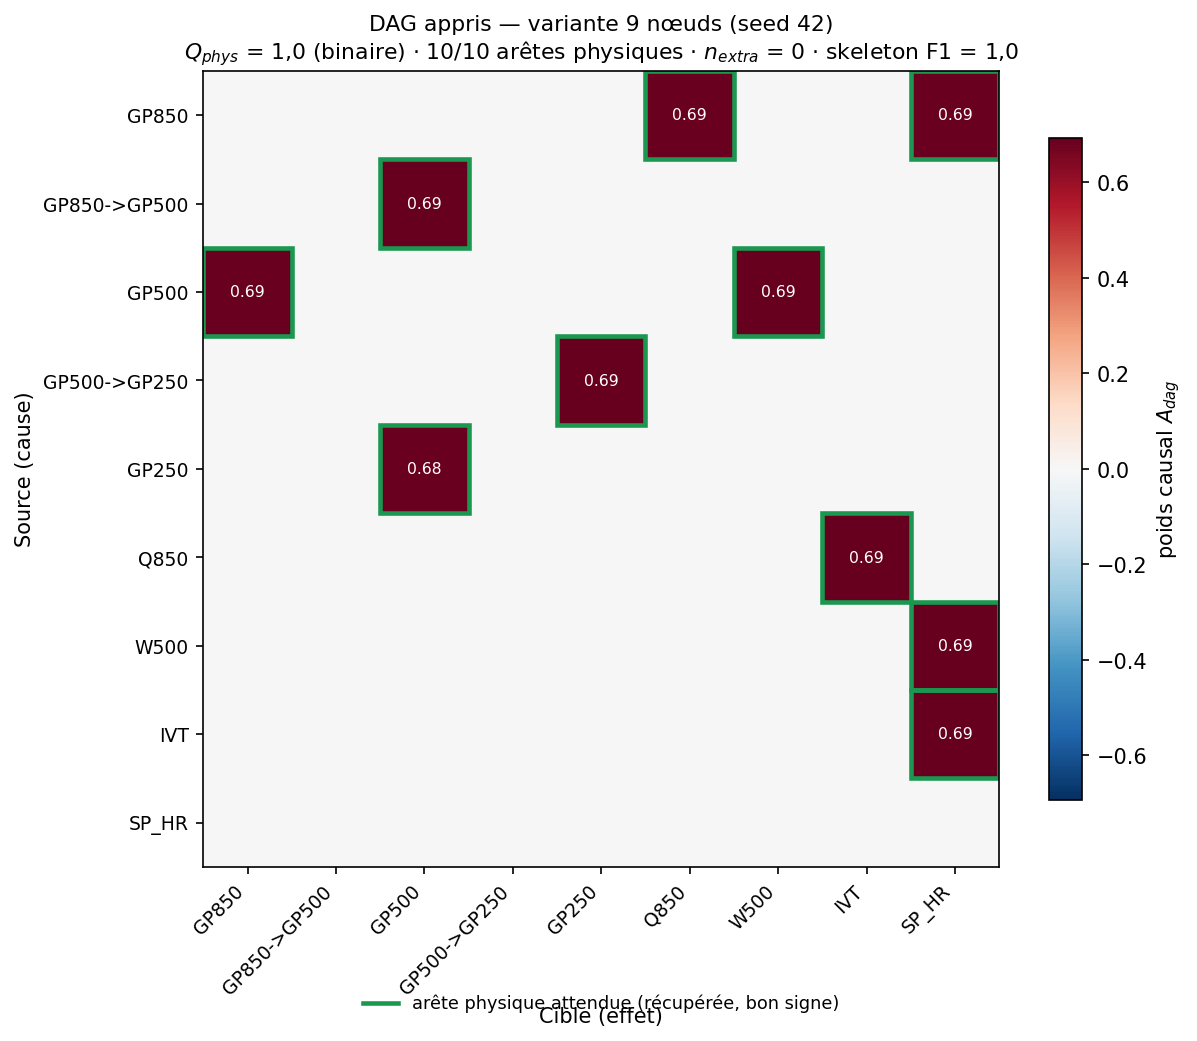
\includegraphics[width=0.72\linewidth]{../results/9node-seed42/annex_dag_heatmap.png}
\caption[DAG appris à 9 nœuds]{Matrice d'adjacence causale $\Adag$ apprise (variante 9 nœuds, seed 42 ; ligne = cause, colonne = effet). Les dix arêtes physiquement attendues (encadrées) sont toutes récupérées avec le signe correct, sans arête parasite.}
\label{fig:exp-9node-dag}
\end{figure}

\begin{table}[H]
  \centering
  \small
  \caption[Arêtes du DAG à 9 nœuds]{Arêtes physiquement attendues et poids appris de $\Adag$ (variante 9 nœuds, seed 42). Les dix arêtes sont récupérées avec le signe correct.}
  \label{tab:exp-9node-edges}
  \begin{tabular}{l c c}
    \toprule
    \textbf{Arête (cause $\to$ effet)} & \textbf{Signe attendu} & \textbf{Poids appris} \\
    \midrule
    GP250 $\to$ GP500          & $+$ & $+0{,}685$ \\
    GP500 $\to$ GP850          & $+$ & $+0{,}688$ \\
    GP850 $\to$ SP\_HR         & $+$ & $+0{,}686$ \\
    GP850$\to$GP500 $\to$ GP500 & $+$ & $+0{,}690$ \\
    GP500$\to$GP250 $\to$ GP250 & $+$ & $+0{,}694$ \\
    GP850 $\to$ Q850           & $+$ & $+0{,}685$ \\
    GP500 $\to$ W500           & $+$ & $+0{,}691$ \\
    Q850 $\to$ IVT             & $+$ & $+0{,}693$ \\
    W500 $\to$ SP\_HR          & $+$ & $+0{,}692$ \\
    IVT $\to$ SP\_HR           & $+$ & $+0{,}692$ \\
    \bottomrule
  \end{tabular}
\end{table}

Cette récupération parfaite de la topologie confirme que la platitude à 6 nœuds n'est pas un plafond de l'architecture, mais le coût d'une agrégation choisie pour la lisibilité ; ce gain de fidélité se paie néanmoins en \emph{skill} de downscaling (Tableau~\ref{tab:exp-6vs9}), ce qui justifie de conserver la configuration à 6 nœuds comme modèle principal.

\myRestoreMarks
